\chapter{INTRODUCTION}
\section{Background}
\label{sec:background} %pelabelan ini opsional, biar bisa di klik kalo mengarahkan ke section tertentu.
\noindent Partial differential equations (PDE) are a common tool widely used in the modern scientific understanding and many engineering processes. This is because many systems can be described by the way they change and often this can be more intuitive. As an example, when cooking with a frying pan on a stove top that is too small, notice that parts of the pan closer to the burner or heating element would heat up faster and stay hotter compared to the edge even after it stops heating up any further and reach a stable temperature. However, a more useful way to describe the system is using the heat equation. For a temperature function $u\left(\vb{x},t\right)$ of spatial coordinates vector $\vb{x}$ and time $t$, the heat equation is defined in \cref{eq:heat_equation}.
\begin{equation} \label{eq:heat_equation}
    \pdv{u}{t}=\alpha\laplacian u
\end{equation}
The Laplacian $\laplacian$ denotes sum of all second spatial derivatives. In three dimensions this is $\laplacian\cdot=\pdv{\cdot}{x_1}+\pdv{\cdot}{x_2}+\pdv{\cdot}{x_3}$. The constant $\alpha$ denotes how fast the heat spreads. Intuitively this equation says that the rate at which the temperature changes in time $\pdv{u}{t}$ is proportional to how different the temperature of a spot in the pan with its surroundings. One example of an insight this gives is that given the stove heat stays constant the temperature will no longer change for a particular point once the temperature difference is constant or in other words the function $u\left(\vb{x},t\right)$ approaches a linear function in space. Mathematically this is because of the Laplacian being second spatial derivatives. Intuitively, once the temperature distribution approaches linear, the current spot on the pan is outputting as much heat it is getting.

Many other systems such as waves, quantum dynamics, fluid dynamics, elastics, and many more also define systems using PDEs. PDEs are also used outside of the physical sciences. In Finance, the Black-Scholes-Merton or Black-Scholes equation models the dynamics of the financial market. In ecology, PDEs are used to model population growth which is usefull for modelling location dependent carrying capacity. This is used to model species distribution which can help develop better conservation policies. In the social sciences, PDEs such as the cross-diffusion model is used to explore the evolution of the urban environment <https://doi.org/10.1038/s41598-023-38979-w>. Crowd dynamics is another field where researchers have found it useful to model using PDEs <https://doi.org/10.1016/S0378-4754(00)00228-7, https://doi.org/10.1109/TSMC.2015.2389763>. These are used to model dynamics such as shock-waves, pathing, and crowd flow as a whole. There are a variety of applications, ranging from brid flocks, pedestrian crowds, to robotic swarms <https://doi.org/10.1146/annurev-control-060822-123629>.


Traditional numerical solvers used to solve PDEs have enjoyed many decades of development due to their long history. There are many general approaches to solve PDEs and many more very specific approaches. Some widely used approaches include Finite Element Methods (FEM), Finite Difference Methods (FDM), and Spectral Methods. FEM and FDM both are mesh based, meaning they rely on discretization of the computational domain <ADD DIAGRAM FOR THIS>. There are several challenges associated with this. First, irregular domains such as bone, spider silk, gravel, or other bio-inspired/aggregate materials,  pose a challenge due to the complexity of the domain geometry <https://doi.org/10.1016/0955-7997(91)90014-K, https://doi.org/10.1016/j.jcp.2007.03.025, https://doi.org/10.1038/s41467-024-47831-2>. Another issue is large deformations or mesh entanglement cause these methods to become ineffective <10.1061/(ASCE)EM.1943-7889.0001176>. While there are strategies to mitigate this, by deffinition they are an additional layer of difficulty to the process. Second, multi-scale applications where the micro and macro scales are both important require fine meshes such that the small scale structures are addequately simulated. This creates very large meshes that are very resource intensive <https://doi.org/10.1016/j.jcp.2007.03.025>. Therefore, in problems where these issues important, meshfree methods are prefered. One approach are Spectral methods which utilize basis functions to approaximate a global solution. A popular choice especially problems with known periodicity, are the Fourier Series. Another drawback of traditional methods are the requirement that PDEs and equations to solve be known analytically. This is because the solvers use the equations to formulate the solution. A dealbreaker like this makes traditional numerical approaches unsuited to data dominant problems. Third, a single evaluation of traditional solvers may not be very costly, multiple evaluations can add up. This is very apparent in inverse problems and other applications where multiple evaluations of the solver is required.

With the increasing prevalance of machine learning methods and their use in more and more fields, research into their use for scientific computing has taken off in recent years. While statistical modeling has already been widely used in areas such as physical constants, stellar population studies, risk assesments of events such as earthquakes and coronal mass ejections <geophysics constants: 10.1029/2002JD002865, CME: https://doi.org/10.1016/j.asr.2005.04.089, asteroid: https://doi.org/10.1111/risa.12453, physics constants: https://doi.org/10.1103/RevModPhys.75.403, http://dx.doi.org/10.1214/074921706000000419, stellar population: https://doi.org/10.1093/mnras/stac3287>, the most widespread approach for forward modeling or inverse modeling are physics based numerical models. With the rise of machine learning methods research into their use for solving PDEs have also expanded.

Another aproach to this starts by viewing PDEs as operators, which are generalized mappings between spaces. Familiar operators are functions which are mappings spaces of scalar values or vector values. PDEs on the other hand are operators that map between function spaces. A simple example is the derivative. It takes in a function and returns the derivative of said function. In other words it is an operator that maps between the space of all functions to the space of derivatives of those functions. Another way to view this is by imagining functions as infinite dimensional vectors. Where elements in the vector are the function's value evaluated at every point. The operator can be seen as vector functions mapping between these infinite dimensional vector spaces. Operators are important because a field of research has sprung up around this mathematical concept. Operator learning is the use of machine learning to learn operators from a data driven approach. As an analogy, regression traditionally has been used to approximate the mapping of functions. In the case of operator learning, a mapping between functions may be approximated.

\noindent Non-destructive testing (NDT) is critical process in the field of engineering and quality assurance that allows the evaluation of a subject without causing damage \autocite{howell2020nondestructive, maioUltrasoundPropagationComposite2022, bochudSparseDigitalSignal2015}. This makes NDT crucial in many cases like construction and manufacturing where testing needs to be done on products without damaging it. The use of NDT allows for early detection of flaws and anomalies ensuring the reliability, longevity, and safety of structures and machinery. A widely used form of NDT, ultrasonic testing, propagates mechanical waves into the material. The ultrasonic waves, typically in the kHz to MHz range, travel through the material and interact with inhomogeneities in the material ie. waves reflected by a cavity. This makes it possible to determine the location, size, and nature of deformities by analyzing the waves measured at predetermined locations. The measurements themselves result in a time series of wave amplitudes represented as displacement. The data can be presented as shown in \Cref{fig:us_presentation}. The amplitude time series by itself is referred as an A-Scan. B-Scans take measurements at multiple locations to show a cross section of the subject. C-Scans adds another dimension of measurements and presents a view of things that reflect the waves such as defects. Analysis of the ultrasonic data can then be carried out. When the material can be assumed homogeneous, ray based or time of flight based methods can be used. In pulse echo, the wave travels through the material and gets reflected by interfaces, whether the other side of the material, fractures within, or generally modulus/density discontinuities present in the material. This means the measurements would record a large amplitude initially from the impulse sent into the material. And then the reflected waves from the closest interface would arrive. This way, just by knowing the exact wave speed of the material, one could easily translate reflected wave arrival time into the positions of interfaces.

\begin{figure}[ht]
    \centering
    \includesvg[inkscapelatex=false, width=1.0\linewidth]{gambar/us scan presentations}
    %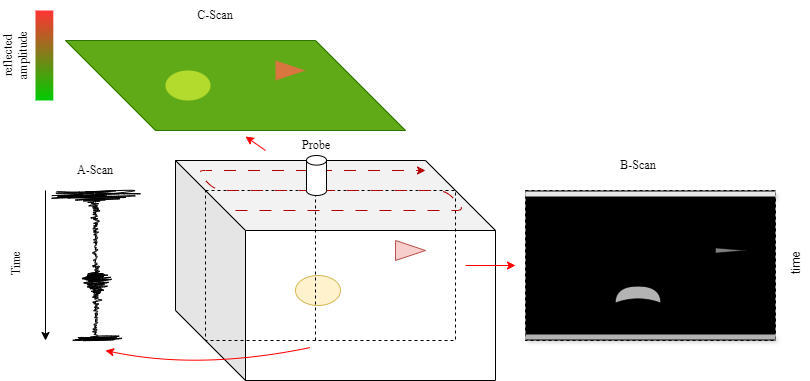
\includegraphics[width=1.0\linewidth]{gambar/us scan presentations.png}
    \caption{Different presentations of ultrasonic scan data. The subject is a box containing several anomalies indicated by the yellow oval and red triangle. The fist presentation is the A-Scan where the amplitude measured over time in one location. The second is B-Scan where the amplitudes over time is measured along a line. The results are then stacked with the vertical axis acting as time and the horizontal axis as position. The higher amplitudes correspond to lighter pixels. The third presentation is C-Scan which is a view of the amplitudes of reflected waves except the initial impulse and back wall reflection.}
    \label{fig:us_presentation}
\end{figure}

Ultrasonic NDT has advantages that makes it one of the more widely used NDT methods \autocite{howell2020nondestructive, nivenFullWaveformInversion2020, feliceSizingFlawsUsing2018}. One advantage is that ultrasonic testing equipment is often portable making it suitable for cases where it is difficult or not possible to test in a controlled environment such as a laboratory. Inspections for infrastructure such as pipes or rail tracks are examples where it is costly and very disruptive to move the test subject to a testing location \autocite{}. Another advantage of ultrasonic testing is the low risk it poses in terms of safety. Unlike the ionizing radiation used in radiography, ultrasonic waves used in testing are harmless to humans. This means testing can be done with relatively less stringent safety precautions \autocite{}. Additionally, the technology is relatively mature with a variety of equipment and supplier options. Furthermore, affordable options for inexpensive ultrasonic equipment is also available \autocite{}. These advantages and the popularity of ultrasonic testing stemming from the aforementioned advantages highlights the important role ultrasonic testing plays in enabling affordable and reliable engineering.

%Talk about the process of A-scans, B-scans, C-scans. Talk about why its hard to analyze for more complex situations which are gaining popularity ie. composites.

The emergence of composites, sought after for their multi-functional properties, introduces challenges for inspection and analysis \autocites{inceOverviewEmergingHybrid2023, yangUltrasonicDetectionMethods2023, dwivediAdvancesResearchesNon2018, nivenFullWaveformInversion2020}. Different composites provide a range of benefits, from the strength to weight ratio of carbon fiber reinforced polymer composites to electromagnetic shielding materials. However, the anisotropic and complex characteristic of composites that give rise to the beneficial properties complicates wave propagation because of the location and directional dependence of material properties. For example wave speed can be faster in certain directions and locations. Reflections will happen not just because of anomalies, but also expected features in the material itself. Extraneous signals from inhomogeneities anticipated in the material makes it harder to extract useful information on unknown defects. In order to enable reliable use of ultrasonic NDT on composite materials and other complex situations, a method to quantify and characterize the complicated behavior is required \autocite{maioUltrasoundPropagationComposite2022}.

This is where model based methods come into play. Advances in computation over recent decades has enabled the use of computational tools to revolutionize many fields. Numerical modeling, in particular, has an almost symbiotic relationship with the rise of computing; with the likes of ENIAC, MANIAC, and a plethora of other early electronic digital computers \autocite{andersonScientificUsesMANIAC1986}. The ENIAC for example, promised to compute ballistic trajectories 10 times faster than the methods that were in used at the time. This progress allows the simulation and analysis of systems previously beyond reach. The effects range from prediction of weather systems and physics constrained problems like bleeding edge aerospace design to uncovering physical laws of nature.

Despite advances in computing power, numerical modeling of physical systems still remains an open problem with many challenges. Traditional methods such as Finite Element Method (FEM), Finite Difference Method (FDM), and Spectral Methods are limited to known operators and equations \autocite{karniadakisPhysicsinformedMachineLearning2021, du2024neural,fanaskovSpectralNeuralOperators2023,luLearningNonlinearOperators2021}. The modern data landscape further complicates traditional numerical modeling with its characteristic abundance of low quality, high quantity data, as some methods such as FDM are inherently sensitive to noise \autocite{dearagaoExplicitControlNumerical2021, huntulInverseProblemReconstructing2021}. Noisy data also presents a formidable challenge in general because gleaning any meaningful information from noisy and incomplete data requires further filtering and interpretation. This issue is particularly troubling for inverse problems. This is because some inverse problems are unstable in addition to their ill-posedness which necessitates advanced techniques \autocite{caubetInstabilityInverseProblem2013, mandacheExponentialInstabilityInverse2001}. The next layer of complexity is posed by the challenge of irregular domains. An example of this is fluid flow through materials such as gravel, sponges, even changing with time \autocite{liImmersedInterfaceMethod2006}. Due to the nature of irregular domains, mesh based methods struggle to adapt. Addressing these challenges is crucial for understanding a variety of problems in both scientific research and engineering.

%talk more about each challenge and the proposed solutions to it and how they do not fully cover the needs this work is trying to cover
The problem posed by model-based ultrasonic testing combines several of these challenges. First, visualizing properties of materials such as density from measurements of ultrasonic waves that interacted with the material is an inverse problem. This is because the effect is used to infer the cause. The challenge with inverse problems is that in many cases, the result is very sensitive to differences in the parameters \autocite{tarantolaInverseProblemTheory2005}; small variation in density distribution can result in very different measurements. As such, additional noise or inaccuracies in measurement can massively impact the predicted parameter. This very issue has been a long standing challenge in the geophysics community. The full waveform inversion (FWI) procedure used to determine properties of the earth, requires certain techniques such as a minimization criteria that mitigates this sensitivity \autocite{virieuxOverviewFullwaveformInversion2009}. Second, complex or irregular domains are a challenge for traditional mesh based methods as the domain may vary in time \autocite{liImmersedInterfaceMethod2006, burchnerImmersedBoundaryParametrizations2023}. Costly mesh generation hampers the performance of mesh based methods. In addition, some approaches like total focusing method (TFM), traveltime tomography (TT) and reverse time migration (RTM) are not able to provide more than a rough estimate of defects. Third, for some materials, there are little to no knowledge present in literature on how waves propagate through the material. Continued research has alleviated this issue by advanced our understanding of wave propagation and materials. \textcite{gordoaUltrasonicWavesBubbly2021} presented an analytic solution to ultrasonic wave propagation in bubbly liquids. \textcite{} . However, these solutions are not available for all situations and materials, as such is the case when a novel material is created. In some of these cases data collection may be easier to do compared to deriving from first principles.

%Talk about how composites, ndt, rapid prototyping, bigalow inflatable space habitat, etc is important to aerospace
Advances in computing technology and the integration of non-destructive testing have revolutionized the aerospace industry \autocite{guptaAdvancesApplicationsNonDestructive2022, jacobDataFusionEfficient2022}. This has had the effect of enabling rapid advancements in cutting-edge technologies such as vertical rocket landings, 3-D printed spacecraft, and in-space manufacturing to name a few \autocite{corradoSpaceExplorationEconomic2023}. These technologies addressed several key challenges with space exploration, namely cost, mission flexibility \& resilience, and environmental considerations. NDT plays a crucial role in ensuring the safety and quality of the innovations. The novelty of innovations means they do not have the luxury of being a proven solution.

%Talk about related works, using conventional methods, using nn, using other machine learning methods, using spectral methods.

Bagian ini mendeskripsikan gambaran umum, konteks, dan posisi penelitian TA dalam konstelasi perkembangan pengetahuan yang telah dicapai. Penjelasan yang dituliskan menjadi penting karena dengan landasan yang kuat, maka pekerjaan penelitian dapat terarah dilakukan. Hal ini lebih spesifik dan tegas disampaikan pada sub-sub bab berikutnya.

Beberapa pustaka utama yang berperan dominan dapat disampaikan di sini untuk memberi gambaran tentang letak penelitian TA dalam konstelasi keilmuan yang dicapai. Hasil-hasil dari pustaka terbaru dapat menopang Latar Belakang ini menjadi lebih kuat.

Sangat wajar apabila isi sub bab setelah Latar Belakang ini mengalami penyesuaian saat sejumlah hasil penelitian sudah diperoleh dan dianalisis. Pada dasarnya, hal ini dimungkinkan apabila ada penyesuaian kecil, karena fokus penelitian sejatinya sudah jelas sedari awal, namun hasil-hasil yang diperoleh dapat memperbaharui beberapa butir isi sub bab. Oleh karena itu, finalisasi isi Pendahuluan ini biasanya dilakukan menjelang akhir pembuatan laporan penelitian yang dituangkan dalam buku TA.


\section{Rumusan dan Batasan Masalah}
\noindent Bagian ini menjadi salah satu bagian penting dalam Pendahuluan. Setelah paparan Latar Belakang, maka masalah yang diangkat pada pekerjaan penelitian perlu dirumuskan dengan baik. Perumusan ini sebaiknya dibahasakan tidak dalam bentuk kalimat pertanyaan, melainkan kalimat aktif, dan dapat memuat lebih dari satu rumusan.

Sejalan dengan ini, setiap masalah yang diangkat selalu memiliki batas. Ada batasan, asumsi, atau kriteria yang menjadi pembatas atas masalah yang diangkat dalam penelitian TA, sehingga arah penelitian dapat fokus. Batasan ini perlu dituliskan secara tegas, dan dapat saja memuat lebih dari satu.


\section{Tujuan}
\label{sec:tujuan}
Bagian ini secara tegas menuliskan tujuan pekerjaan penelitian TA, yang dapat memuat lebih dari satu. Pemilihan kata kerja pada Tujuan ini sangat penting karena menggambarkan arah fokus dari jalinan upaya yang dilakukan.


\section{Metodologi}
Di sini disampaikan metodologi yang diterapkan pada pekerjaan penelitian TA. Beberpa di antaranya adalah pengamatan dan akuisisi data, eksperimen numerik, studi pustaka, teoretik atau analitik, dan semi analitik dengan komplemen numerik.



\section{Sistematika Penulisan}
\noindent Bagian ini adalah penutup Bab I yang menyampaikan  secara ringkas isi setiap  bab. Karena pembaca sudah sampai akhir Bab I, yang  berarti  sudah  mengetahui isinya, maka tidak perlu ditulis lagi rincian Bab I. Sebaiknya langsung dituliskan secara ringkas isi rincian bab-bab selanjutnya, misalnya, \textit{Setelah Pendahuluan pada Bab I ini, Bab II akan mengulas tentang ...}

Apabila diperlukan, dapat dituliskan konvensi khusus yang digunakan pada penulisan naskah buku TA ini, misalnya tanda titik menggantikan tanda desimal karena alasan kemudahan dan kejelasan dalam formulasi matematika.